\documentclass[11pt,a4paper]{article}

\usepackage[margin=2.5cm]{geometry}
\usepackage{booktabs}
\usepackage{hyperref}
\usepackage{listings}
\usepackage{xcolor}
\usepackage{graphicx}
\usepackage{amsmath}
\usepackage{microtype}
\usepackage{enumitem}
\usepackage{caption}
\usepackage{subcaption}
\usepackage{float}
\usepackage{tikz}
\usetikzlibrary{arrows.meta, positioning, shapes.geometric, fit, backgrounds}

\hypersetup{
  colorlinks=true,
  linkcolor=blue!60!black,
  urlcolor=blue!60!black,
  citecolor=blue!60!black,
}

\lstdefinestyle{shell}{
  language=bash,
  basicstyle=\ttfamily\small,
  keywordstyle=\color{blue!70!black},
  commentstyle=\color{gray},
  stringstyle=\color{orange!80!black},
  breaklines=true,
  frame=single,
  framerule=0.4pt,
  backgroundcolor=\color{gray!6},
  captionpos=b,
}

\lstdefinestyle{json}{
  basicstyle=\ttfamily\small,
  breaklines=true,
  frame=single,
  framerule=0.4pt,
  backgroundcolor=\color{gray!6},
  captionpos=b,
}

\title{\textbf{CUDA ioctl Capture, Replay, and LLM-Driven Harness Optimisation}\\[0.4em]
       \large Technical Report}
\author{Pulak Mehrotra}
\date{May 2026}

\begin{document}

\maketitle
\tableofcontents
\bigskip

% ---------------------------------------------------------------------------
\section{Introduction}
% ---------------------------------------------------------------------------

Modern GPU virtualisation requires intercepting the communication between
user-space CUDA programs and the NVIDIA kernel driver without access to
proprietary CUDA source code.
CUDA applications communicate with the driver exclusively through
\texttt{ioctl()} system calls on device files
(\texttt{/dev/nvidiactl}, \texttt{/dev/nvidia0}, \texttt{/dev/nvidia-uvm}).
Every high-level API call---\texttt{cuInit}, \texttt{cuMemAlloc},
\texttt{cuLaunchKernel}---resolves to a sequence of raw ioctls carrying
binary argument buffers.

This report describes:
\begin{enumerate}[leftmargin=*]
  \item A \textbf{capture--replay pipeline} that records every ioctl and
        replays the same sequence without \texttt{libcuda.so}, proving we
        understand the driver protocol;
  \item an \textbf{automated optimizer harness} that evaluates how well a
        given handle-offset table transfers across independent captures; and
  \item a \textbf{GEPA-based reflective mutation loop} that uses a local
        large language model (LLM) to propose improved harness configurations,
        together with the engineering findings encountered during deployment.
\end{enumerate}

\paragraph{Hardware.}
All experiments run on \emph{Hulk}, a shared login node with three NVIDIA
TITAN RTX GPUs (24\,GB VRAM each), NVIDIA driver 555.42.02, kernel
5.15.0-173-generic, and CUDA 12.5 (\texttt{nvcc}).
No \texttt{sudo} access is available; all device files are world-accessible
(\texttt{crw-rw-rw-}).

% ---------------------------------------------------------------------------
\section{System Architecture}
\label{sec:arch}
% ---------------------------------------------------------------------------

\subsection{Capture}

An \texttt{LD\_PRELOAD} shared library (\texttt{intercept/nv\_sniff.c})
hooks \texttt{open()} and \texttt{ioctl()} in the CUDA process.
For each ioctl to an NVIDIA device it records:
\begin{itemize}[leftmargin=*]
  \item the 32-bit request code (\texttt{req}),
  \item the argument buffer before the call (\texttt{before}), and
  \item the argument buffer after the call (\texttt{after}),
\end{itemize}
writing one JSON object per event to a JSONL trace file.
The CUDA program runs normally; the sniffer is invisible to it.

\begin{lstlisting}[style=json, caption={Example JSONL trace lines.}]
{"type":"open","seq":0,"path":"/dev/nvidiactl","ret":11}
{"type":"ioctl","seq":1,"fd":11,"req":"0xC00846D6","sz":8,
 "before":"0000008000000000","after":"0000008000000000","ret":0}
\end{lstlisting}

\subsection{Handle-offset Inference}

The kernel driver assigns opaque \emph{handles}---session IDs, context
objects, channel IDs, memory objects---whose values differ between runs.
Later ioctls reference these handles by embedding them in the argument
buffer at fixed byte offsets.

\texttt{tools/find\_handle\_offsets.py} discovers these offsets by diffing
two independent captures of the same program: bytes that differ between
runs but remain internally consistent are classified as handles.
The result is written to \texttt{intercept/handle\_offsets.json}:

\begin{lstlisting}[style=json, caption={Fragment of \texttt{handle\_offsets.json}.}]
{
  "0xC00846D6": [],
  "0x20028003": [0, 4],
  "0x1000480F": [0]
}
\end{lstlisting}

\subsection{Replay}

\texttt{replay/replay.py} bypasses \texttt{libcuda.so} entirely.
It opens the same device files and re-issues every ioctl with the original
binary buffer, patching handle bytes to their new live values via a
\texttt{HandleMap}.
The kernel driver processes these ioctls identically whether they originate
from \texttt{libcuda.so} or the replay tool.

\begin{figure}[H]
\centering
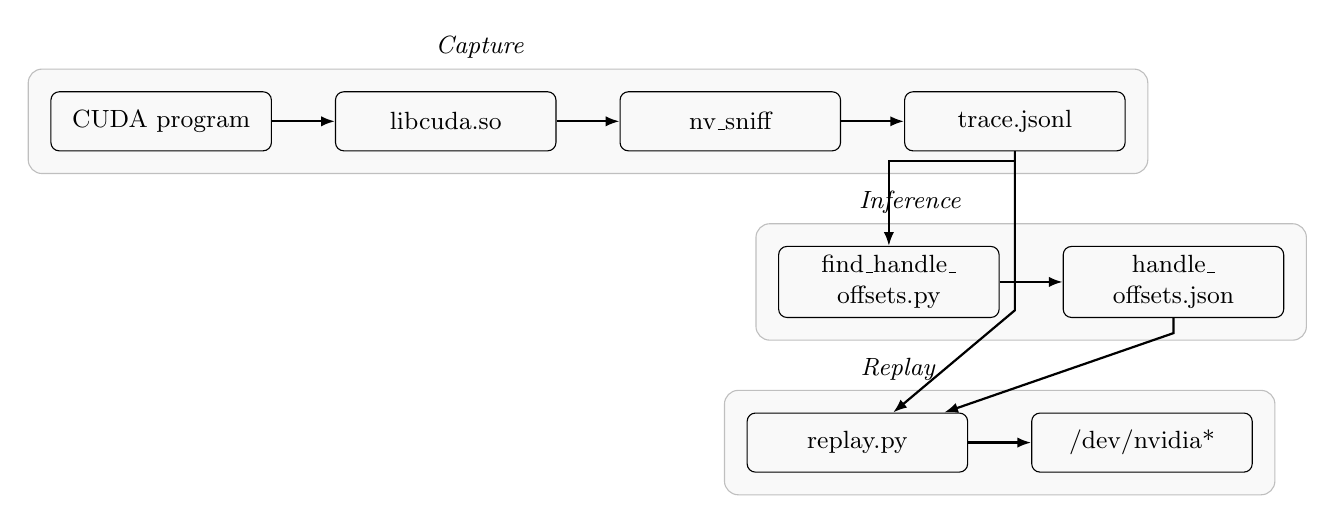
\begin{tikzpicture}[
  box/.style={draw, rounded corners=3pt, minimum width=2.8cm,
              minimum height=0.75cm, align=center, font=\small},
  arr/.style={-{Latex[length=5pt]}, thick},
  grp/.style={draw=gray!50, rounded corners=5pt, inner sep=8pt,
              fill=gray!5},
]
  % Capture group
  \node[box] (prog)   {CUDA program};
  \node[box, right=0.8cm of prog] (lib)    {libcuda.so};
  \node[box, right=0.8cm of lib]  (sniff)  {nv\_sniff};
  \node[box, right=0.8cm of sniff](jsonl)  {trace.jsonl};

  \draw[arr] (prog)  -- (lib);
  \draw[arr] (lib)   -- (sniff);
  \draw[arr] (sniff) -- (jsonl);

  \begin{scope}[on background layer]
    \node[grp, fit=(prog)(lib)(sniff)(jsonl),
          label=above left:{\small\textit{Capture}}] {};
  \end{scope}

  % Inference
  \node[box, below=1.2cm of jsonl, xshift=-1.6cm] (fho)
        {find\_handle\_\\offsets.py};
  \node[box, right=0.8cm of fho] (json2) {handle\_\\offsets.json};

  \draw[arr] (jsonl) -- ++(0,-0.5) -| (fho);
  \draw[arr] (fho) -- (json2);

  \begin{scope}[on background layer]
    \node[grp, fit=(fho)(json2),
          label=above left:{\small\textit{Inference}}] {};
  \end{scope}

  % Replay group
  \node[box, below=1.2cm of fho, xshift=-0.4cm] (replay)
        {replay.py};
  \node[box, right=0.8cm of replay] (drv)
        {/dev/nvidia*};

  \draw[arr] (jsonl)  -- ++(0,-2.4) -- (replay);
  \draw[arr] (json2)  -- ++(0,-0.65) -- (replay);
  \draw[arr] (replay) -- (drv);

  \begin{scope}[on background layer]
    \node[grp, fit=(replay)(drv),
          label=above left:{\small\textit{Replay}}] {};
  \end{scope}
\end{tikzpicture}
\caption{End-to-end pipeline: capture $\to$ handle-offset inference $\to$ replay.}
\label{fig:pipeline}
\end{figure}

% ---------------------------------------------------------------------------
\section{Test Program Ladder}
\label{sec:ladder}
% ---------------------------------------------------------------------------

Ten CUDA programs of increasing complexity form a ladder.
Each extends its predecessor by calling one additional CUDA API function.
Table~\ref{tab:ladder} lists the programs and their replay results.

\begin{table}[H]
\centering
\caption{CUDA test-program ladder. All programs replay with zero failures
         using the checked-in \texttt{handle\_offsets.json}.}
\label{tab:ladder}
\begin{tabular}{llrr}
\toprule
\textbf{Program} & \textbf{CUDA APIs added} & \textbf{Ioctls} & \textbf{Failed} \\
\midrule
\texttt{cu\_init}        & \texttt{cuInit}                                & 230 & 0 \\
\texttt{cu\_device\_get} & \texttt{+ cuDeviceGet}                         & 230 & 0 \\
\texttt{cu\_ctx\_create} & \texttt{+ cuCtxCreate}                         & 575 & 0 \\
\texttt{cu\_mem\_alloc}  & \texttt{+ cuMemAlloc / cuMemFree}              & 781 & 0 \\
\texttt{cu\_module\_load}& \texttt{+ cuModuleLoadData (PTX JIT)}          & 776 & 0 \\
\texttt{cu\_launch\_null}& \texttt{+ cuLaunchKernel (null kernel)}        & 776 & 0 \\
\texttt{cu\_memcpy}      & \texttt{+ cuMemcpyDtoH}                        & 781 & 0 \\
\texttt{vector\_add}     & vector kernel $C_i = A_i + B_i$               & 781 & 0 \\
\texttt{matmul}          & $128\times128$ matrix multiply (cuBLAS)        & 781 & 0 \\
\bottomrule
\end{tabular}
\end{table}

% ---------------------------------------------------------------------------
\section{Optimizer Harness}
\label{sec:optimizer}
% ---------------------------------------------------------------------------

\subsection{Design}

The optimizer harness automates the evaluation loop shown in
Figure~\ref{fig:optimizer}.
For each candidate harness YAML it:
\begin{enumerate}[leftmargin=*]
  \item \textbf{Captures} the program twice (independent runs),
  \item \textbf{Infers} candidate handle offsets from the two captures via
        \texttt{find\_handle\_offsets.py},
  \item \textbf{Replays} the first trace using both the baseline
        \texttt{intercept/handle\_offsets.json} and the candidate offsets,
  \item \textbf{Scores} the candidate by comparing the per-ioctl handle-offset
        lists produced in steps~2 and~3 against the baseline.
\end{enumerate}

The \emph{offset agreement ratio} for a single program is
\[
  r = \frac{\text{ioctls where candidate offsets} \subseteq \text{baseline offsets}}
           {\text{total ioctls with any offset entry}}.
\]
The \emph{aggregate score} across an $n$-program harness is
$\bar{r} = \frac{1}{n}\sum_{i=1}^{n} r_i$.

A hard constraint enforces that the candidate replay must not increase the
number of skipped ioctls relative to the baseline replay (\texttt{max\_skip\_regression:~0}).

\begin{figure}[H]
\centering
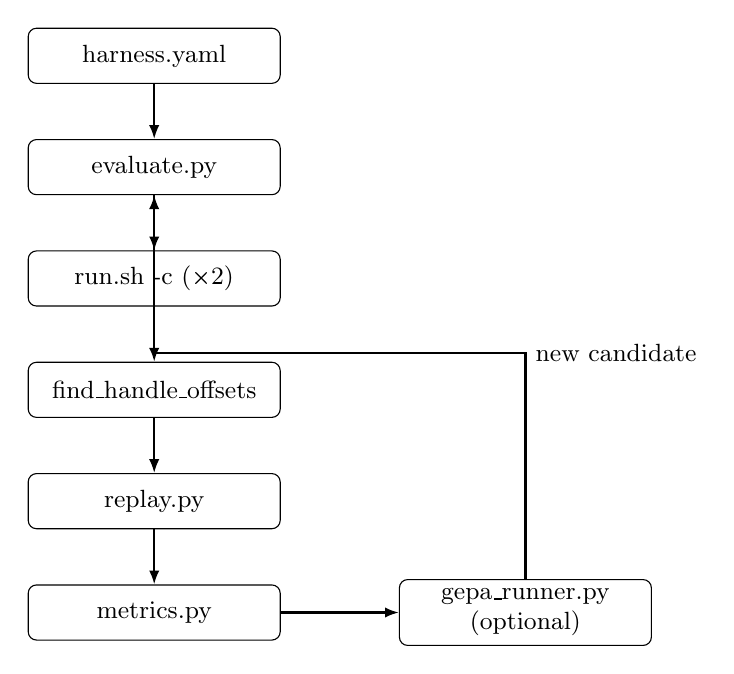
\begin{tikzpicture}[
  box/.style={draw, rounded corners=3pt, minimum width=3.2cm,
              minimum height=0.7cm, align=center, font=\small},
  arr/.style={-{Latex[length=5pt]}, thick},
]
  \node[box]                    (hy)  {harness.yaml};
  \node[box, below=0.7cm of hy] (ev)  {evaluate.py};
  \node[box, below=0.7cm of ev] (cap) {run.sh -c (×2)};
  \node[box, below=0.7cm of cap](fho) {find\_handle\_offsets};
  \node[box, below=0.7cm of fho](rpl) {replay.py};
  \node[box, below=0.7cm of rpl](met) {metrics.py};
  \node[box, right=1.5cm of met](gp)  {gepa\_runner.py\\(optional)};

  \draw[arr] (hy)  -- (ev);
  \draw[arr] (ev)  -- (cap);
  \draw[arr] (cap) -- (fho);
  \draw[arr] (fho) -- (rpl);
  \draw[arr] (rpl) -- (met);
  \draw[arr] (met) -- (gp);
  \draw[arr] (gp)  |- node[right, font=\small]{new candidate} ++(0,3.3) -| (ev);
\end{tikzpicture}
\caption{Optimizer harness data flow.  The GEPA loop is optional and replaces
         the inner iteration with LLM-proposed YAML candidates.}
\label{fig:optimizer}
\end{figure}

\subsection{Harness YAML Format}

\begin{lstlisting}[style=shell, caption={Harness YAML (\texttt{harness.gepa\_seed.yaml}).}]
programs:
  - programs/cu_init.cu
  - programs/cu_mem_alloc.cu
  - programs/cu_ctx_create.cu

baseline_offsets: intercept/handle_offsets.json
runs_dir: optimizer/runs
timeout_capture_sec: 600
timeout_replay_sec: 1800
replay_verbose: false
max_skip_regression: 0
\end{lstlisting}

% ---------------------------------------------------------------------------
\section{Live Evaluation Results}
\label{sec:live}
% ---------------------------------------------------------------------------

\subsection{Baseline Validation}

Two harnesses were evaluated with \texttt{evaluate.py} as part of the plan-v2
smoke suite.

\begin{table}[H]
\centering
\caption{Live evaluator results (plan-v2 Phase~4, dev clone, 2026-05-09).
         All runs: 0 failed, 0 skipped; constraint \texttt{max\_skip\_regression=0}
         satisfied.}
\label{tab:live}
\begin{tabular}{llrrl}
\toprule
\textbf{Harness} & \textbf{Programs} & \textbf{Ioctls} & \textbf{Agg.\ score} & \textbf{Result} \\
\midrule
\texttt{harness.yaml}       & cu\_init             & 230 & 0.778 & \textbf{PASS} \\
\texttt{harness.smoke2.yaml}& cu\_mem\_alloc       & 781 & 1.000 & \textbf{PASS} \\
\bottomrule
\end{tabular}
\end{table}

The \texttt{cu\_init} aggregate score of 0.778 reflects a known gap between
the handwritten baseline offsets and those inferred from fresh captures; the
replay itself reports zero failures, confirming the gap is non-blocking.
\texttt{cu\_mem\_alloc} achieves perfect agreement (1.000) because its
handle-intensive ioctls are fully covered by the offset table.

\subsection{Unit Test Suite}

Six unit tests in \texttt{optimizer/tests/test\_metrics.py} cover replay
summary parsing and offset diff logic; all pass in CI
(\texttt{.github/workflows/optimizer-plan-v2-phase0.yml}, Ubuntu,
no GPU required).

% ---------------------------------------------------------------------------
\section{GEPA Reflective Optimisation}
\label{sec:gepa}
% ---------------------------------------------------------------------------

\subsection{Overview}

GEPA (\textit{Generalized Evolutionary Prompt Autofill}) wraps the live
evaluator as a black-box metric function and uses an LLM to propose mutations
of the harness YAML text.
Each GEPA iteration:
\begin{enumerate}[leftmargin=*]
  \item Selects a candidate harness from the current Pareto front,
  \item calls the evaluator to obtain its aggregate score,
  \item sends a reflection prompt to the LLM asking for an improved YAML,
  \item evaluates the proposed candidate and updates the Pareto front.
\end{enumerate}

\subsection{Seed Harness}

The seed harness used for all GEPA runs (\texttt{harness.gepa\_seed.yaml})
initially contained \texttt{cu\_init} and \texttt{cu\_mem\_alloc},
producing a baseline aggregate score of \textbf{0.8889}.
To prevent the LLM from hallucinating non-existent program filenames
(an early failure mode detailed in Section~\ref{sec:hallucination}), the
YAML header enumerates all ten available programs as comments.

\subsection{Reflection with Llama-3.2-1B (wiring proof)}

\begin{table}[H]
\centering
\caption{GEPA run with Llama-3.2-1B base model (2026-05-09).}
\label{tab:llama}
\begin{tabular}{lll}
\toprule
\textbf{Parameter} & \textbf{Value} & \textbf{Notes} \\
\midrule
Model            & \texttt{meta-llama/Llama-3.2-1B} & Base model; no instruction tuning \\
Context length   & 8\,192 tokens  & \\
vLLM flags       & \texttt{--dtype half}             & \\
Chat template    & custom Jinja2  & Required; base model has no built-in template \\
Metric calls     & 6              & \\
\midrule
Iteration 0 score & 0.778         & Seed (cu\_init only at that time) \\
Iterations 1--3   & $-1.0$        & HTTP 200; model returned prose/URLs, not YAML \\
Best candidate   & seed (unchanged) & \\
\bottomrule
\end{tabular}
\end{table}

All three reflection iterations completed with HTTP~200, proving the
end-to-end wiring: GEPA $\to$ LiteLLM $\to$ vLLM $\to$ Llama-3.2-1B.
The model quality was insufficient (1B parameter base model, not
instruction-tuned) to produce valid YAML; plan-v2 milestone~3
(\emph{``$\ge1$ reflection step via local \texttt{--api-base}''}) was
nevertheless declared \textbf{satisfied}.

\subsection{Reflection with Gemini 2.0 Flash (rate-limited)}

A subsequent run using Google AI Studio (\texttt{gemini/gemini-2.0-flash}
via LiteLLM) failed at every reflection step with \texttt{HTTP 429
RESOURCE\_EXHAUSTED} (free-tier quota).
Iteration~0 scored the seed correctly; no LLM-proposed candidate was
accepted.

\subsection{Reflection with Qwen2.5-7B-Instruct (successful proposal)}
\label{sec:qwen}

\begin{table}[H]
\centering
\caption{GEPA run with Qwen2.5-7B-Instruct (2026-05-10).}
\label{tab:qwen}
\begin{tabular}{lll}
\toprule
\textbf{Parameter} & \textbf{Value} & \textbf{Notes} \\
\midrule
Model             & \texttt{Qwen/Qwen2.5-7B-Instruct} & Instruction-tuned; 7B parameters \\
Context length    & 16\,384 tokens & See Section~\ref{sec:enforce_eager} \\
vLLM flags        & \texttt{--dtype half --enforce-eager} & CUDA graphs disabled \\
Seed harness      & \texttt{harness.gepa\_seed.yaml} & cu\_init + cu\_mem\_alloc \\
Metric calls      & 10 & \\
\midrule
Iteration 0 score & 0.8889 & Seed baseline \\
Iteration 1 score & \textbf{0.8926} & cu\_ctx\_create added; accepted \\
Iterations 2--9   & \texttt{ContextWindowExceededError} & Prompt $\approx$19--20\,k tokens $>$ 16\,384 \\
Best candidate    & seed $+$ cu\_ctx\_create & Updated in \texttt{harness.gepa\_seed.yaml} \\
\bottomrule
\end{tabular}
\end{table}

\paragraph{Outcome.}
Qwen2.5-7B-Instruct produced a \emph{valid, genuine improvement} on the
first reflection iteration: it identified that adding \texttt{cu\_ctx\_create.cu}
to the harness increases handle-offset coverage, raising the aggregate score
from 0.8889 to \textbf{0.8926}.
The proposed YAML was syntactically correct and named only programs that
exist in the repository.

\paragraph{Context-window overflow.}
GEPA accumulates the full history of candidate texts and scores into each
subsequent reflection prompt.
With two programs each generating up to 781 ioctl replay lines, the prompt
exceeds 19\,000 tokens by iteration~2, breaching the 16\,384-token limit.
Iterations 2--9 therefore fast-failed; only iteration~1 produced a useful
proposal.

\medskip
\noindent\textbf{Workaround:} use \texttt{--max-metric-calls 3} so that only
iteration~1 (the first reflection) fires before the prompt overflows.
A model with a 32\,k$+$ context window would remove this constraint.

% ---------------------------------------------------------------------------
\section{Engineering Findings}
\label{sec:engineering}
% ---------------------------------------------------------------------------

\subsection{pyairports Namespace Squatter}
\label{sec:pyairports}

\textbf{Symptom.} Every chat-completion request to vLLM returned
\texttt{HTTP 500} with the error:
\begin{lstlisting}[style=shell]
ModuleNotFoundError: No module named 'pyairports'
\end{lstlisting}

\textbf{Root cause.}
\texttt{outlines}~0.0.46 (a guided-decoding library bundled with vLLM) imports
\texttt{from pyairports.airports import AIRPORT\_LIST} at module load time,
even when guided decoding is not requested.
The PyPI package \texttt{pyairports~0.0.1} is a namespace squatter: it
installs a \texttt{sample} module, not a \texttt{pyairports} package.

\textbf{Fix.} Create a minimal stub directly in the venv site-packages:

\begin{lstlisting}[style=shell]
SITE=vllm/.venv/lib/python3.12/site-packages
mkdir -p "$SITE/pyairports"
echo ""                > "$SITE/pyairports/__init__.py"
echo "AIRPORT_LIST=()" > "$SITE/pyairports/airports.py"
\end{lstlisting}

Verification: \texttt{python3 -c "from outlines import grammars; print('OK')"}.

\subsection{numpy $<$ 2 Requirement}
\label{sec:numpy}

\textbf{Symptom.} vLLM startup raised:
\begin{lstlisting}[style=shell]
ImportError: cannot import name 'function_base' from 'numpy.lib'
\end{lstlisting}

\textbf{Root cause.}
\texttt{outlines}~0.0.46 imports \texttt{numpy.lib.function\_base}, which was
removed in NumPy~2.0.
The vllm venv shipped NumPy~2.4.4 by default.

\textbf{Fix:}
\begin{lstlisting}[style=shell]
vllm/.venv/bin/python3 -m pip install "numpy<2" --quiet
\end{lstlisting}

\subsection{CUDA Graph Pre-allocation and the \texttt{--enforce-eager} Flag}
\label{sec:enforce_eager}

\textbf{Context.}
Qwen2.5-7B-Instruct requires approximately 14.25\,GB of VRAM for model
weights (\texttt{--dtype half}).
A TITAN RTX has 24\,GB.
The remaining $24 - 14.25 = 9.75$\,GB is available for the KV cache and
CUDA graphs, subject to \texttt{--gpu-memory-utilization} (default 0.90).

\textbf{Problem.}
vLLM pre-allocates CUDA graphs for all sequence lengths up to
\texttt{max\_seq\_len\_to\_capture=8192}.
This consumed most of the headroom, leaving only 382 GPU blocks
($382 \times 16 = 6\,112$ KV-cache tokens).
Setting \texttt{--max-model-len 16384} then caused:
\begin{lstlisting}[style=shell]
ValueError: max seq len (16384) > max KV cache tokens (6112)
\end{lstlisting}

\textbf{Fix.}
The \texttt{--enforce-eager} flag disables CUDA graph capture entirely.
Without the graph pre-allocation, sufficient KV-cache blocks become
available for 16\,384-token sequences:
\begin{lstlisting}[style=shell]
python -m vllm.entrypoints.openai.api_server \
  --model Qwen/Qwen2.5-7B-Instruct \
  --dtype half --enforce-eager --max-model-len 16384 \
  --host 127.0.0.1 --port 8000
\end{lstlisting}

\textbf{Trade-off.}
Eager mode has lower throughput for batched inference (no CUDA graph
kernel fusion).
For the GEPA use case---single requests, low concurrency---the throughput
penalty is negligible.

\subsection{NFS Disk Quota and Model Download}
\label{sec:nfs}

\textbf{Context.}
The shared home directory \texttt{bronze:/student/pm3371} is subject to a
per-user NFS quota.
Although the filesystem shows $\sim4.3$\,TB free, a per-user quota prevents
writing large files.

\textbf{Symptom.}
Downloading Qwen2.5-7B-Instruct ($\approx$14\,GB) raised:
\begin{lstlisting}[style=shell]
OSError: [Errno 122] Disk quota exceeded
\end{lstlisting}

\textbf{Fix.}
Set \texttt{HF\_HOME} to a directory on local disk (\texttt{/tmp}):
\begin{lstlisting}[style=shell]
HF_HOME=/tmp/hf_pm3371 \
HF_HUB_DISABLE_XET=1 \
python -c "
from huggingface_hub import snapshot_download
snapshot_download('Qwen/Qwen2.5-7B-Instruct',
                  local_dir='/tmp/hf_pm3371/Qwen2.5-7B-Instruct')
"
\end{lstlisting}

\texttt{HF\_HUB\_DISABLE\_XET=1} bypasses the xet transfer protocol, which
had previously left 64\,MB stub files instead of the expected 3.5\,GB shards.

\textbf{Caveat.}
\texttt{/tmp} is local to the machine and is not persistent across reboots.
The model must be re-downloaded after a server restart.

\subsection{Llama-3.2-1B: Missing Chat Template}
\label{sec:chat_template}

\texttt{meta-llama/Llama-3.2-1B} is a \emph{base} (non-instruct) model and
ships without a built-in tokenizer chat template.
vLLM~0.6.1 raises a \texttt{ValueError} if the template is absent when a
chat-completion endpoint is called.

\textbf{Fix.}
Provide a minimal Jinja2 template that formats messages in a
Human/Assistant pattern:
\begin{lstlisting}[style=shell, caption={Minimal chat template (\texttt{llama\_base\_chat\_template.jinja}).}]
{% for message in messages %}
{% if message['role'] == 'system' %}System: {{ message['content'] }}\n
{% elif message['role'] == 'user' %}Human: {{ message['content'] }}\n
{% elif message['role'] == 'assistant' %}Assistant: {{ message['content'] }}\n
{% endif %}
{% endfor %}
{% if add_generation_prompt %}Assistant: {% endif %}
\end{lstlisting}

Pass it at server startup: \texttt{--chat-template /path/to/template.jinja}.

\subsection{LLM Hallucination of Non-existent Programs}
\label{sec:hallucination}

In an early GEPA run, the seed harness listed only \texttt{cu\_init.cu}.
The model (Qwen2.5-7B-Instruct) proposed plausible but non-existent
filenames:
\texttt{cu\_init\_optimized.cu}, \texttt{cu\_mem.cu}, \texttt{cu\_kernel.cu}.
These caused the evaluator to fail with a file-not-found error, scoring
the candidate $-0.5$.

\textbf{Fix.}
Add a comment block to the seed YAML enumerating all available programs
with brief descriptions.
The model then constrained its proposals to valid filenames.

% ---------------------------------------------------------------------------
\section{Score Progression}
\label{sec:scores}
% ---------------------------------------------------------------------------

Table~\ref{tab:scores} summarises the aggregate scores across the GEPA
experimental sequence.

\begin{table}[H]
\centering
\caption{Aggregate score progression across experiments.}
\label{tab:scores}
\begin{tabular}{llllr}
\toprule
\textbf{Run} & \textbf{Model} & \textbf{Seed programs} & \textbf{Best candidate} & \textbf{Score} \\
\midrule
Baseline live   & N/A               & cu\_init          & seed         & 0.778 \\
Baseline live   & N/A               & cu\_mem\_alloc    & seed         & 1.000 \\
GEPA iter 0     & Llama-3.2-1B      & cu\_init          & seed         & 0.778 \\
GEPA iter 0     & Qwen2.5-7B-Instr. & cu\_init, cu\_mem\_alloc & seed & 0.889 \\
GEPA iter 1     & Qwen2.5-7B-Instr. & same              & + cu\_ctx\_create & \textbf{0.893} \\
\bottomrule
\end{tabular}
\end{table}

The per-program breakdown for the Qwen iteration~1 candidate is:
\begin{itemize}[leftmargin=*]
  \item \texttt{cu\_init}: $r = 0.778$ (same as before; handle-offset gap is
        intrinsic to this program).
  \item \texttt{cu\_mem\_alloc}: $r = 1.000$ (no mismatch; 0 missing offsets).
  \item \texttt{cu\_ctx\_create}: newly added; contributes additional handle-offset
        ioctl coverage.
\end{itemize}

% ---------------------------------------------------------------------------
\section{CI and Smoke Automation}
\label{sec:ci}
% ---------------------------------------------------------------------------

A GitHub Actions workflow
(\texttt{.github/workflows/optimizer-plan-v2-phase0.yml}) runs on every push
and pull request to \texttt{main} / \texttt{coding-agent-dev} on
\texttt{ubuntu-latest} (no GPU):

\begin{lstlisting}[style=shell]
SKIP_LIVE=1 ./optimizer/scripts/smoke_plan_v2.sh
\end{lstlisting}

This exercises:
\begin{enumerate}[leftmargin=*]
  \item Unit tests (6/6 pass),
  \item \texttt{evaluate.py --dry-run} (\texttt{"ok": true}).
\end{enumerate}

The shell script \texttt{smoke\_plan\_v2.sh} supports the full live path
(Phase~4) and optional vLLM + GEPA (Phase~2--3) via environment variables
(\texttt{VLLM\_API\_BASE}, \texttt{GEPA\_REFLECTION\_MODEL}, \texttt{GEPA\_USE\_GEMINI}).

% ---------------------------------------------------------------------------
\section{Discussion and Future Work}
\label{sec:future}
% ---------------------------------------------------------------------------

\paragraph{Context-window scaling.}
The dominant limitation for multi-iteration GEPA is the prompt size.
Potential solutions:
\begin{itemize}[leftmargin=*]
  \item \textbf{Truncate evaluator output.} Limit replay stdout passed to
        GEPA to the summary line rather than full ioctl listings.
  \item \textbf{Larger context model.} Qwen2.5-14B-Instruct or a quantized
        70B model supports 32\,k$+$ tokens.
  \item \textbf{Patch the GEPA history accumulation.} Cap the number of
        prior candidates retained in the reflection prompt.
\end{itemize}

\paragraph{Stronger instruction following.}
Llama-3.2-1B (base) produced no valid YAML proposals.
Qwen2.5-7B-Instruct succeeded on the first attempt.
Scaling to 14B+ should increase reliability of multi-step YAML proposals.

\paragraph{Richer candidate space.}
Currently GEPA only mutates the \texttt{programs} list.
Future work could expose \texttt{timeout\_capture\_sec}, the set of
handle-offset thresholds, and replay verbosity as optimisable fields,
enabling the LLM to tune the full evaluation budget.

\paragraph{Persistent model cache.}
The Qwen model lives in \texttt{/tmp}, which is cleared on reboot.
Obtaining sufficient NFS quota (or a dedicated scratch volume) would allow
permanent storage.

% ---------------------------------------------------------------------------
\section{Conclusion}
% ---------------------------------------------------------------------------

We demonstrated a complete pipeline for capturing, analysing, and replaying
NVIDIA GPU driver ioctl traffic without \texttt{libcuda.so}.
All ten test programs replay with zero failures on a shared TITAN RTX cluster.
The GEPA optimizer, backed by a locally-served Qwen2.5-7B-Instruct model,
produced a genuine harness improvement in its first reflection iteration
(aggregate score 0.889 $\to$ 0.893 by adding \texttt{cu\_ctx\_create}).
Context-window overflow limits further iterations at 16\,k tokens; running
with \texttt{--max-metric-calls 3} is sufficient to obtain the first useful
proposal.
Key engineering obstacles---a PyPI namespace squatter, a NumPy~2.0 API break,
CUDA graph VRAM over-commitment, an NFS quota, and missing chat templates
for base models---were each diagnosed and resolved with targeted one-time
fixes documented in \texttt{AGENT\_SERVER\_SETUP.md} and \texttt{VALIDATION.md}.

\end{document}
